\documentclass{IOS-Book-Article}
\usepackage[utf8]{inputenc}
\usepackage{graphicx}
\usepackage{framed}
\usepackage[normalem]{ulem}

\def\hb{\hbox to 11.5 cm{}}

\newcommand{\sembrack}[1]{[\![#1]\!]}
\newcommand{\subex}[2]{#1_{#2}}
\newcommand{\commentOut}[1]{}
\newcommand{\eop}[1]{\mbox{\textsl{#1}}}
\newcommand{\ttop}[1]{\mbox{\texttt{#1}}}

\newcommand{\bequ}{\begin{quote}}
\newcommand{\enqu}{\end{quote}}
\newcommand{\bece}{\begin{center}}
\newcommand{\ence}{\end{center}}
\newcommand{\todoj}[1]{{\color{red}\textbf{[J: #1]}}}
\newcommand{\todoi}[1]{{\color{magenta}\textbf{[I: #1]}}}

\newenvironment{compactitem}{\begin{itemize}}{\end{itemize}}

\begin{document}

\pagestyle{headings}
\def\thepage{}
\begin{frontmatter}              % The preamble begins here.

\title{An End-to-End Pipeline from Law Text to Logical Formulas}

\markboth{}{September 2022 - Anonymised Review Copy\hb}

% \author[A]{Aarne Ranta}
% \author[B,C]{Inari Listenmaa}
% \author[C]{Jerrold Soh}
% \author[C]{Meng Weng Wong}

% \address[A]{
%   Department of Computer Science and Engineering,
%   Chalmers University of Technology and University of Gothenburg,
%   aarne.ranta@cse.gu.se
%   }
% \address[B]{Digital Grammars}
% \address[C]{Centre for Computational Law, Singapore Management University}

\begin{abstract}
 This paper develops a pipeline for converting natural English law texts into logical formulas via a series of structural representations. The goal is to study how law-to-logic translation can be achieved with a sequence of well-defined steps. The texts are first parsed using a formal grammar derived from light-weight text annotations designed to minimise the need for manual grammar construction. An intermediate representation, called assembly logic, is then used for logical interpretation and supports translations to different back-end logics and visualisations. The approach, while rule-based and explainable, is also robust: it can deliver useful results from day one, but allows subsequent refinements and variations. While some work is needed to extend the method to new laws, the software presented here reduces the marginal effort necessary. As a case study, we demonstrate our approach on one part of Singapore’s Personal Data Protection Act. Our code is available open-source.
\end{abstract}

\begin{keyword}
legal formalisms, legal text parsing, Grammatical Framework, context-free grammars, methodology
\end{keyword}
\end{frontmatter}
\markboth{September 2022 - Anonymised Review Copy\hb}{September 2022 - Anonymised Review Copy\hb}

%\maketitle
\section{Introduction}

Expressing laws computably is a classic objective of AI \& Law \cite{mccarty_reflections_1977, sergot_british_1986} and a crucial pre-requisite to automating downstream tasks such as compliance checking \cite{palmirani_modelling_2018, hickey_gdpr_2021}, policy support \cite{svensson_expertisze_1992, haan_tracs_1992}, information retrieval \cite{bing_designing_1987}, argumentative reasoning \cite{mochales_study_2008}, legislative simulation \cite{bench-capon_logic_1987, bench-capon_support_1992}, and formal verification \cite{haan_tracs_1992}. But faithfully translating law to logic is challenging, often requiring expertise in both legal and formal methods. This ``natural language barrier'' \cite{mccarty_deep_2007} poses a significant ``knowledge bottleneck'' \cite{nazarenko_pragmatic_2021} to the development of computational law systems. Thus, numerous strategies have been devised for bridging the barrier. These include domain-specific ontologies \cite{palmirani_legal_2018}, taxonomies \cite{hulstijn_taxonomy_2020}, vocabularies \cite{hickey_gdpr_2021}, standards \cite{sartor_akoma-ntoso_2011}, logics \cite{prakken_logical_1993}, markup languages \cite{athan_oasis_2013}, and programming languages \cite{huttner_catala_2022}, intermediate formalisms for expressing laws \cite{mccarty_language_1989, kralingen_norm_1993, mccarty_deep_2007}, as well as specialised human workflows \cite{palmirani_legal_2018, witt_converting_2021}.

Early in the field's history, \cite{bing_designing_1987} had already imagined automatic parsers for translating natural language laws into formal logic programs. Several steps have since been taken towards that vision. For instance, McCarty \cite{mccarty_deep_2007} demonstrated how \cite{collins_head-driven_2003}'s statistical parser can extract, from judicial opinion texts, syntax trees which may then be converted into quasi-logical semantic representations of said texts using definite clause grammars. Others have examined how far machine learning methods can implicit learn or represent legal principles and concepts \cite{groendijk_neural_1992, de_maat_automatic_2008, winkels_automatic_2012, chalkidis_neural_2019, chalkidis_lexglue_2022}. However, the NLP framework chosen often constrains the translation process (see e.g.\ \cite{quaresma_question_2005}). In particular, whether the chosen framework accommodates the logic representation desired is not always clear \cite{wyner_study_2013}.

This paper contributes to this literature by describing a partially-automated law to logic pipeline based on Grammatical Framework (GF, \cite{ranta-2011}). Prior legal applications of GF \cite{angelov-al-2013, gdpr-2018} have typically focused on Controlled Natural Languages (CNL, e.g.\ \cite{fuchs-al-2008, angelov-ranta-2009}).
Our approach is novel in that we tackle real-world law texts. Nonetheless, we exploit features of GF which have proven fruitful for CNL processing: modularity, precision, and support for semantic back-ends via an abstract syntax. One limitation of GF is that writing GF grammars requires specialised expertise. To counteract this, we develop a method for automatically extracting a preliminary grammar from light-weight annotations which non-experts can create. The preliminary grammar is usable as-is for a rough analysis of law texts but can be gradually improved by manual refinement. Overall, this approach requires less effort than writing grammars from scratch. Our code is available open-source.\footnote{URL to be provided here after blind review.}

Section \ref{sec:methods} details our pipeline. Section \ref{sec:pdpa} exemplifies the pipeline using a case study on Singapore's \textit{Personal Data Protection Act} 2012 (PDPA). Section \ref{sec:discussion} discusses future directions and concludes.

\section{Methodology}
\label{sec:methods}

\begin{figure}[h!]
    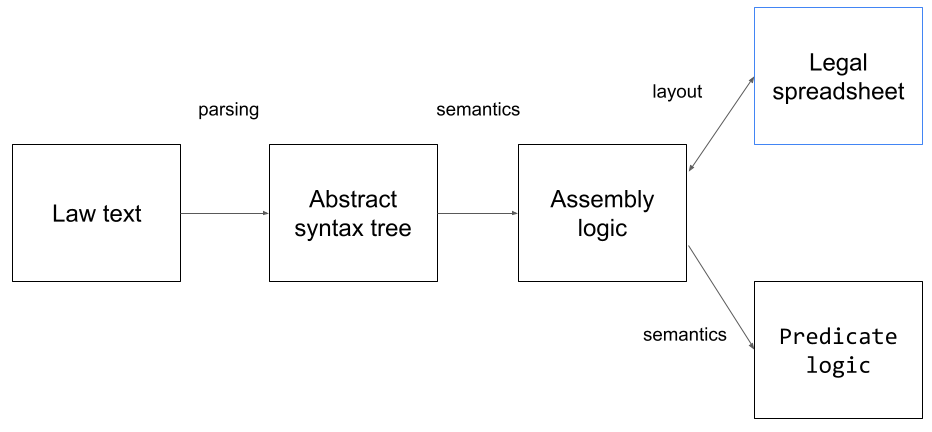
\includegraphics[width=0.8\textwidth]{pipeline.png}
\caption{The pipeline}
\label{pipeline}
\end{figure}

\subsection{Pipeline Overview}

Figure~\ref{pipeline} provides an overview of the pipeline. The primary input is a statutory text in natural language which we assume has been properly extracted and tokenised by some standard tool such as GF's \texttt{lextext} converter.
The resulting \texttt{.txt} is converted to abstract syntax trees (ASTs) line by line using the GF parser driven by a grammar (see Section \ref{sec:2.2}). 
The ASTs are then converted into an intermediate representation we call assembly logic (Section \ref{sec:assembly-logic}) using the Haskell-based methodology described in \cite{ranta-2011c}. Assembly logic is more abstract than the ASTs from the parser, but preserves more distinctions than standard back-end logics.
These distinctions are useful for deriving different output formats such as predicate logic (Section \ref{sec:predicate-logic}) and visualisations (Section \ref{sec:vis:spreadsheets}).

% , while Fig.\ref{pipeline-ex} shows a concrete example of its use on a paragraph of text.
% The second step is converting the abstract syntax trees resulting from the parser into formulas in an \textbf{assembly logic}.
% This is an intermediate representation between abstract syntax trees and normal ``back end'' logics such as predicate logic.
% It is more abstract than the syntax trees coming from the parser, but preserves more distinctions than, say, predicate logic.
% These distinctions are particularly useful when deriving visualizations of the structure, such as \textbf{spreadsheets}, two-dimensional representations that make the logical structure explicit without using logical formulas.
% These visualizations are intended to help understand the text and also to select proper interpretations of it in case of ambiguity.
% The conversion is performed in Haskell using the methodology described in \cite{ranta-2011c}.

% context-free grammar automatically derived from the text itself.
% At a later phase, we can optionally replace this with a richer kind of GF grammar.

% the structure, such as \textbf{spreadsheets}, two-dimensional representations that make the logical structure explicit without using logical formulas.
% These visualizations are intended to help understand the text and also to select proper interpretations of it in case of ambiguity.
% The conversion is performed in Haskell using the methodology described in \cite{ranta-2011c}.

\subsection{From Law Text to ASTs}
\label{sec:2.2}

The primary legal texts are first converted into ASTs using GF \cite{ranta-2011}, a special-purpose programming language for grammar development. 
In typical GF applications, the ASTs are intended for further processing such as translations to other natural languages or to logical semantics.
GF grammars are usually written by hand to guarantee precise correspondence to the desired ASTs.
Nonetheless, GF's extensive Resource Grammar Library (RGL, \cite{ranta-2009}), which implements the basic syntax and morphology of over 40 languages, reduces the manual effort necessary.

Not surprisingly, however, the RGL is not sufficient for legal purposes. The constructs covered by the RGL are limited to single utterances; parsing law texts commonly requires handling long itemised lists and paragraphs. As these syntactic constructs are significant for law's logical structure, we wanted the parser to capture them appropriately.
Thus, we developed a tailored grammar for our purposes using the RGL as a base.
We began building the grammar in a data-driven, top-down manner, starting from entire lines of text and going forward by stepwise refinement of the grammar rules.
To this end, we developed a semi-automatic method where a Haskell script generates GF rules from manual annotations of the source text.
Figure~\ref{grammar-gen} illustrates the grammar building workflow.

\begin{figure}[h!]
 \begin{framed}
\bequ
\textbf{A line in the raw text:}
\bequ
\textit{(2) without limiting subsection (1)(a), a data breach is deemed to result in significant harm to an individual ---}
\enqu
\textbf{The line annotated with marks for terminals} (\verb6#6) \textbf{and nonterminals} (\verb6*6):
\bequ
\begin{verbatim}
*Item (2) #without #limiting #subsection *Ref (1)(a) #,
#a *CN data breach #is #deemed #to
*VP result in significant harm to an individual #-
\end{verbatim}
\enqu
\textbf{Grammar rules derived automatically by the script:}
\bequ
\begin{verbatim}
Line ::= Item "without" "limiting" "subsection" Ref ","
         "a" CN "is" "deemed" "to" VP "-" ;
Item ::= "(2)" ;
Ref  ::= "(1)(a)" ;
CN   ::= "data" "breach" ;
VP   ::= "result" "in" "significant"
         "harm" "to" "an" "individual" ;
\end{verbatim}
\enqu
\textbf{The VP rule above manually refined into more general rules:}
\bequ
\begin{verbatim}
VP2 ::= "result" "in" NP ;
NP  ::= "significant" "harm" "to" NP ;
NP  ::= "an" CN ;
CN  ::= "individual" ;
\end{verbatim}
\enqu
\textbf{The same four rules converted into GF abstract syntax functions:}
\bequ
\begin{verbatim}
fun VP2_result_in : VP2 ;
fun CN_significant_harm_to_NP : NP -> CN ;
fun NP_an_CN : CN -> NP ;
fun CN_individual : CN ;
\end{verbatim}
\enqu
\textbf{Manually merging morphological variants (with rules derived elsewhere):}
\bequ
\sout{\texttt{fun CN\_individuals : CN ;}} \\
\texttt{fun CN\_individual : CN ;} {\it --- automated choice of singular vs. plural}
\sout{\texttt{fun NP\_an\_CN : CN -> NP ;}} \\
\texttt{fun NP\_a\_CN  : CN -> NP ;} {\it --- automated choice of `a' vs. `an'}
\enqu
\enqu
\end{framed}
\caption{The grammar extraction process.}
\label{grammar-gen}
\end{figure}

The script produces a BNF (context-free) grammar in a notation usable in GF as-is.
Internally, GF then automatically adds to each rule an abstract syntax function whose name is derived from items in the rule itself.
The final GF grammar is more expressive and more abstract than BNF and can merge morphological variants of rules. As Figure~\ref{grammar-gen} shows, \verb6CN_individual6 can be merged with \verb6CN_individuals6 (which is derived from a different part of the source text).
The automatically derived functions only cover the respective strings ``individual'' and ``individuals'', but the manually merged function covers both the singular and plural forms.
Similarly, \verb6NP_an_CN6 can be merged with \verb6NP_a_CN6.
An advantage, in addition to having fewer rules, is that the choice of the singular and the plural, or \textit{a} vs.\ \textit{an}, can then be made precisely depending on the context.

\subsection{From ASTs to Assembly Logic}
\label{sec:assembly-logic}

Assembly logic is an intermediate representation between ASTs and standard logics.
It is designed to preserve enough of the raw texts' syntactic structure to generate alternative forms recognizable by humans as representations of the original text.
For example, it distinguishes between ordinary and reverse implications (``if A then B'' vs.\ ``B if A'').
It also preserves quantified noun phrases as units (e.g.\ ```any organization'') and is neutral as to how modalities (e.g.\ ``must'', ``may'') are formalised.
At the same time, it is intended to be sufficient to represent more varied sets of ASTs, so that when the grammar is extended (e.g.\ via annotations of new law texts), the assembly logic and its back-ends can be kept constant.

Figure~\ref{assembly} shows a sample of the assembly logic implemented as a Haskell datatype \texttt{Formula}.
It also shows part of an \textbf{interpretation function} \cite{ranta-2011c}, \texttt{iNP}, which converts ASTs of GF type \texttt{NP} (Noun Phrase) to assembly logic.
These functions use pattern matching over trees.
Each AST constructor may have its own pattern, such as for \verb6NP_any_CN6 in Figure~\ref{assembly}.
When the grammar is extended, new patterns can be added.
But even if this is not done, the function can take care of the new constructors by the catch-all case (\verb6_6) which treats the new expressions as atomic.
Atomic expressions can then be converted to atomic formulas or constants in logics and to single cells in spreadsheets (see Section~\ref{sec:vis:spreadsheets}).

\begin{figure}
  \begin{framed}
 \bequ
 \textbf{Some assembly logic constructors:}
 \enqu

\bequ
\begin{verbatim}
  data Cat =
    CProp | CSet | CInd | ...
  data Formula =
    Atomic Cat Atom
  | Conjunction Cat ConjWord [Formula]
  | Implication Formula Formula
  | Conditional Formula Formula     -- reverse implication
  | Quantification String Formula   -- quantifier + domain
\end{verbatim}
 \enqu
 \bequ
 \textbf{Semantics of ASTs in the assembly logic:}
\enqu
\bequ
\begin{verbatim}
  iNP :: Env -> NP -> Formula
  iNP env np = case np of
    NP_any_CN cn -> Quantification "ANY" (iCN env cn)
    NP_each_CN cn -> Quantification "EACH" (iCN env cn)
    ...
    _ -> Atomic CInd (toAtom env np) -- convert to string
\end{verbatim}
 \enqu

   \end{framed}
\caption{Data structures and conversions related to the assembly logic.}
\label{assembly}
\end{figure}

\subsection{From Assembly Logic to Predicate Logic}
\label{sec:predicate-logic}

Assembly logic is then mapped into a many-sorted logic with Russell's iota terms. In turn, the many-sorted logic is mapped into ordinary predicate logic and rendered in TPTP \cite{sutcliffe2009tptp} notation. 
We use many-sorted logic because it better supports compositional translation.
Thus quantification expressed by noun phrases (e.g.\ ``any storage medium'') are compositionally interpreted as quantifiers with sorts rather than divided into unsorted quantifiers and sort predicates.
The sorts are eliminated during the conversion from many-sorted to ordinary predicate logic.

More importantly, anaphoric expressions (e.g.\ ``that organization'') are interpreted as definite descriptions formalised as iota terms. (We write $\iota(A)$ instead of $(\iota x)A(x)$, leaving possible variable bindings to $A$ itself, as is customary in higher-order logic.)
These iota terms are eliminated in a pass that looks for non-iota terms in their context of use.
Figure~\ref{anaphora} illustrates this using the well-known ``donkey sentence'' \cite{geach-1962,kamp-1981}: ``if a man owns a donkey he beats it.''
This sentence has an existential quantifier in the antecedent and a pronoun or definite description referring to it in the succedent.
To express this reference in ordinary predicate logic, the existential quantifier is changed into a universal one with a wide scope of implication.

\begin{figure}
  \begin{framed}
  \bequ
    \textbf{A donkey sentence inspired by our case study below:}
    \bequ
        \textit{if a notification is a data breach, the notification is affected}
    \enqu

    \textbf{Compositional interpretation in many-sorted logic with iota terms:}
\[
(\exists x : \eop{notification})\eop{data\_breach}(x) \, \supset \, \eop{affected}(\iota(\eop{notification}))
\]

    \textbf{Conversions to ordinary predicate logic in TPTP notation:}
    \bequ
        \begin{verbatim}
![X]:(notification(X) => data_breach(X) => affected(X))
        \end{verbatim}
    \enqu
    \enqu
    \end{framed}
 \caption{Iota terms are eliminated via anaphora resolution.}
\label{anaphora}
\end{figure}

Donkey sentences are ubiquitous in law texts, as in many other types of text.
Interestingly, inverted donkey sentences --- where the existential appears in the succedent and is referred to in the antecedent --- also occurred in our sample text. Figure~\ref{donkey} shows an example of one such sentence undergoing the conversion to many-sorted logic and thereafter TPTP. Note that the TPTP output is not guaranteed to be error-free and still requires manual checking.

\begin{figure}
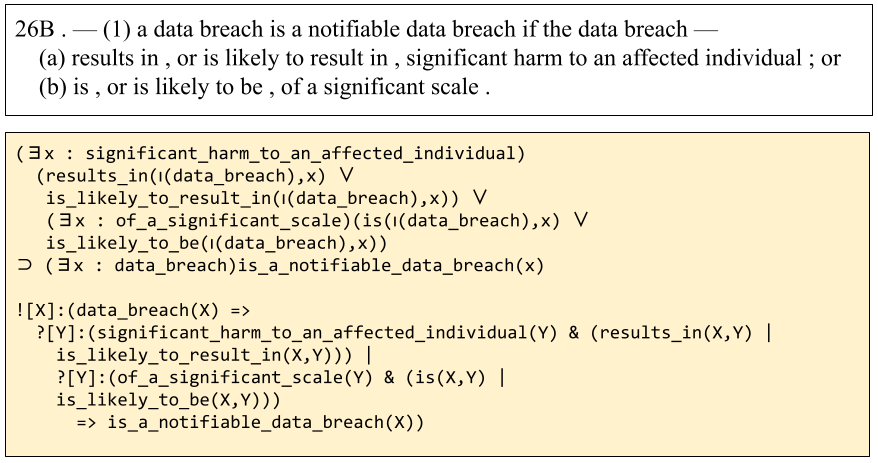
\includegraphics[width=0.96\textwidth]{anaphora.png}
\caption{An inverted donkey sentence from the actual law text undergoing similar treatment.}
\label{donkey}
\end{figure}

\subsection{From Assembly Logic to Spreadsheets}
\label{sec:vis:spreadsheets}

The AST can also be automatically visualised in a spreadsheet (see Figure \ref{pipeline-ex}) displaying the formula trees in a structured format (like in \cite{mochales_study_2008}). The spreadsheet format, which serves as the input to a low-code programming platform, is currently under development and will be more fully described in future work.

\section{Formalizing the Personal Data Protection Act}
\label{sec:pdpa}

We illustrate our pipeline using Part 6A of the PDPA. Like the EU's \textit{General Data Protection Regulation} (GDPR), the PDPA is Singapore's primary data protection statute and prescribes obligations surrounding the collection, use, disclosure, and deletion of personal data. Part 6A stipulates when and how organisations are expected to notify regulators of data breaches. We use the PDPA as a case study for three reasons. First, this was a practical suggestion from Singapore's Personal Data Protection Commission (who hypothesised that formalizing the PDPA would help them better manage legislative change).
Second, while the PDPA has not been examined in AI \& Law literature, its subject matter connects it to prior work on the GDPR \cite{palmirani_modelling_2018,palmirani_legal_2018,hickey_gdpr_2021}.
Third, Part 6A is complex enough to demonstrate the utility of a computational law approach in general and our pipeline in particular. Indeed, modelling these rules allowed us to detect a race condition in the PDPA: an organisation which informed both the Commission and the affected individuals of a data breach, as s~26D PDPA generally requires, might inadvertently violate s~26D(6) which provides that organisations should \textit{not} inform affected individuals if the Commission so directs.

Table \ref{stats} provides a statistical summary of our raw PDPA text. Given space constraints, Figure \ref{pipeline-ex} below illustrates the pipeline on a selected portion of Part 6A. A complete parse of Part 6A into ASTs, assembly logic, and spreadsheets may be found on our repository. The assembly logic to TPTP conversion is also complete save for two assembly logic formulas which contain nominalised modalities --- we will address this in future work.

\begin{table}[h!]
  \begin{tabular}{|l|r|}
\hline
        
lines & 47 \\
characters & 5964 \\
tokens & 1053 \\
unique tokens & 228 \\
tokens per line on average & 22 \\
tokens on the longest line & 56 \\
\hline
  \end{tabular}
  \caption{Statistics on Part 6A PDPA}
  \label{stats}
  \vspace{-8mm}
\end{table}

\begin{figure}
    \bequ
    \textbf{A paragraph in the raw text:}
    \enqu
    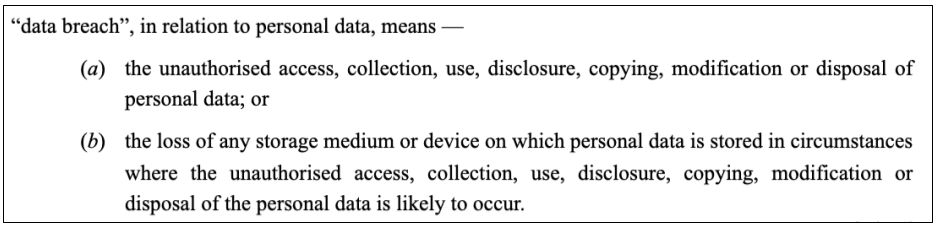
\includegraphics[width=0.7\textwidth]{text.png}

    \bequ
    \textbf{AST of line (a):}
    \enqu
    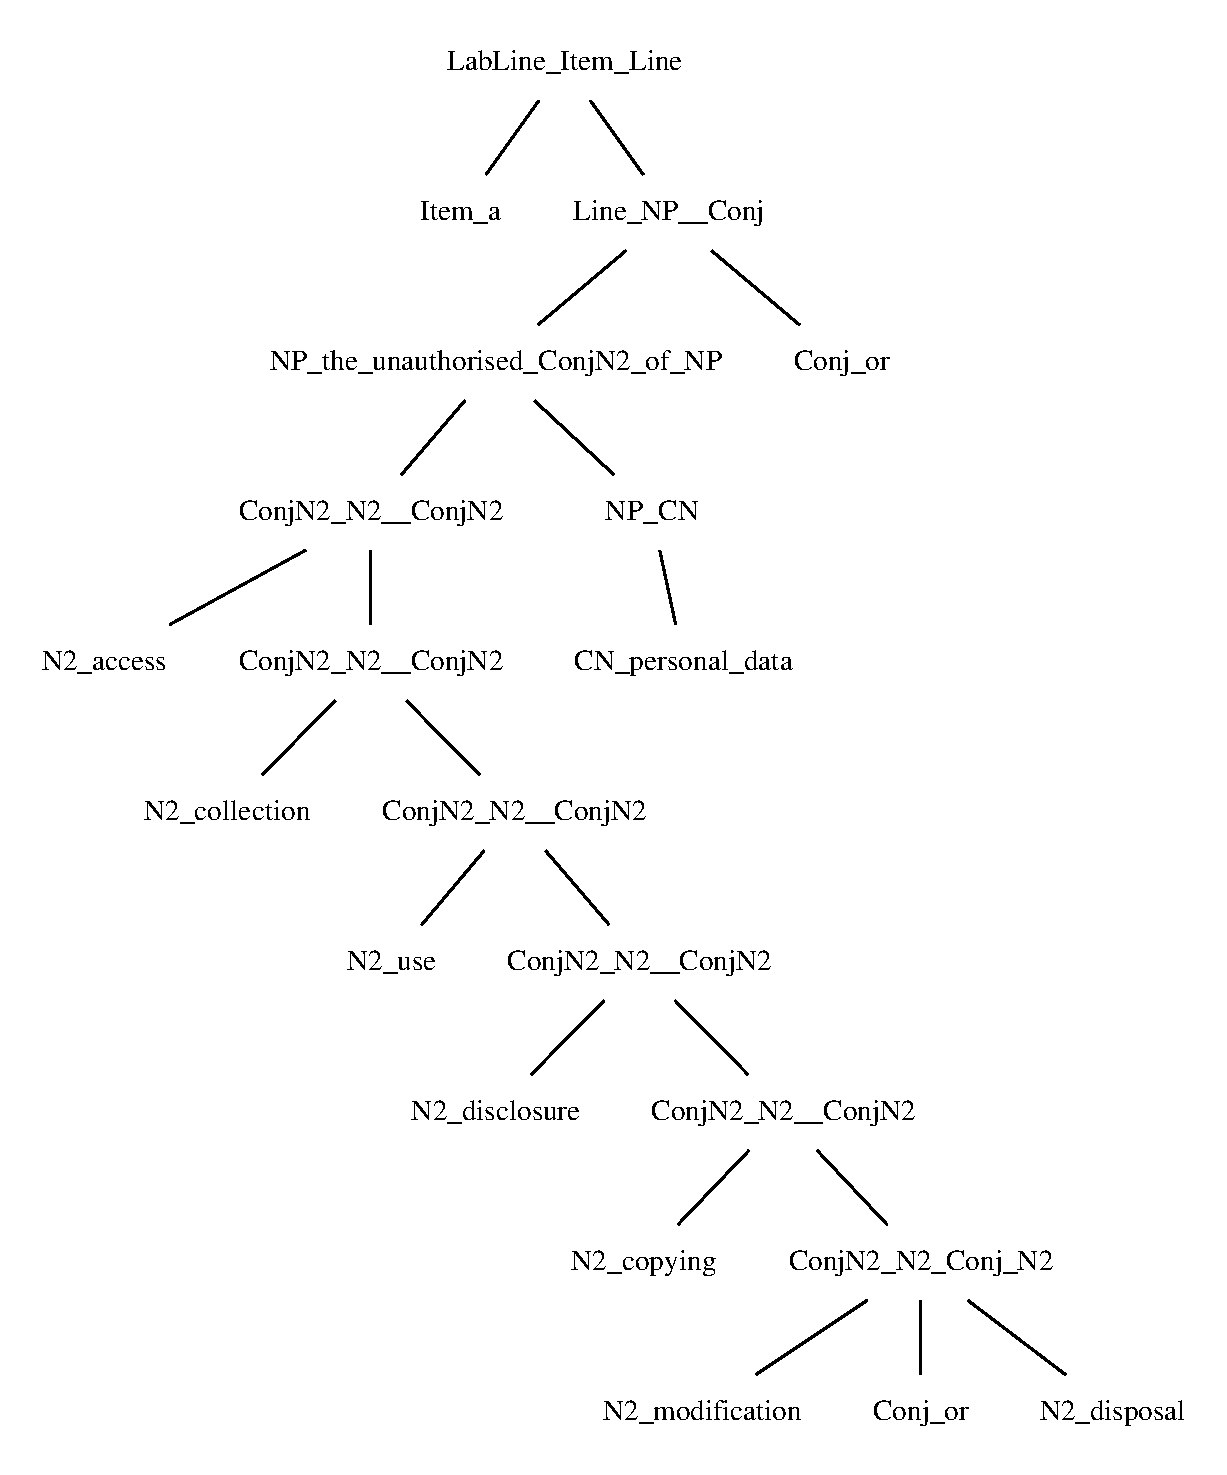
\includegraphics[width=0.5\textwidth]{tree.eps}
      \bequ
      \textbf{TPTP notation of the full paragraph:}
      \enqu
    \bequ
    \small
    \begin{verbatim}
  ![X]:(data_breach(X) & ?[Y]:(personal_data(Y) & IN_RELATION_TO(X,Y)) <=>
  (personal_data(X) & ?[Y]:((access(Y,X) | collection(Y,X) | use(Y,X) |
  disclosure(Y,X) | copying(Y,X) | modification(Y,X) | disposal(Y,X)) &
  unauthorized(Y))) | (((storage_medium(X) | device(X)) & (personal_data(X) &
  ?[Y]:((circumstances(Y) & (((unauthorized(Y) & (access(Y) | collection(Y) |
  use(Y) | disclosure(Y) | copying(Y) | modification(Y) | disposal(Y))) &
  is_likely_to_occur(Y))) & is_stored_in(X,Y)))) & loss(X))))
    \end{verbatim}
    \enqu

    \normalsize
    \bequ
    \textbf{Visualised in a spreadsheet}
    \enqu
    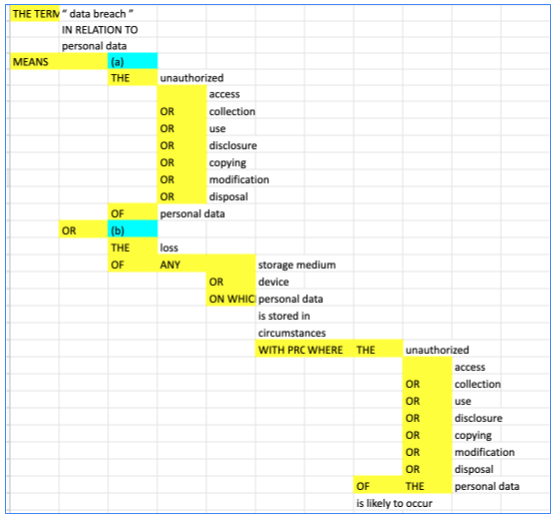
\includegraphics[width=0.4\textwidth]{assembly.png}
\caption{An example through the pipeline: text, abstract syntax tree (of the second line), spreadsheet, and formula in TPTP notation.}
\label{pipeline-ex}
\end{figure}

\section{Conclusion}
\label{sec:discussion}
Converting law to logic is a known hard problem. In this paper our goal was to examine how a sophisticated linguistic framework like GF could help with the process. To this end, we developed a GF-based pipeline that parses legal text into ASTs, assembly logic, and thereafter predicate logic. That such a pipeline was successfully developed demonstrates the promise of this approach. While manual effort was still required at various stages, the process was less tedious than a completely manual one. More importantly, some pipeline steps can work out of the box when the input scope is extended. Others, such as the the text annotations for extending the grammar and the conversion to assembly logic, are light-weight enough to make the system feasible to apply to new texts. Further, since GF's mapping between ASTs and natural language is fully reversible, the pipeline can be easily extended to support natural language generation. Once parsed into GF trees, the source text can be modified into novel forms: declarative sentences can become questions, negations, hypotheticals, etc. 

There remain a few limitations which we hope future work can address. First, the amount of manual checking necessary to refine the intermediate grammars and output logic remains substantial. This did not surprise us given the enormity of the law-to-logic challenge, but it should be possible to optimise the pipeline further (e.g.\ by writing scripts to automatically merge compatible grammar rules in the preliminary, automatically extracted grammar). Second, we have not verified the accuracy and representativeness of our PDPA formalisation (this itself being a standard challenge in this area, see \cite{wyner_study_2013}). We aim to eventually compare logical outputs generated by our approach against gold standards developed by human legal and technical experts and vetted by the relevant regulatory body. The legal language barrier is far from solved, but we hope to have taken one more step towards realising that vision.

% Future papers will link this pipeline with other work at CCLAW: on the spreadsheet syntax, the logical semantics, and the grammar of smaller units.

% \todoj{feel free to condense this paragraph into as few words as you like!}

% The GF trees are so far used to parse text. However, the manually refined rules (merging singular and plural, `a` vs. `an` from Figure~\ref{grammar-gen}) carry all potential for generating natural language output: the more general and powerful grammar knows when to \textit{output} a singular or plural form, guaranteeing a grammatically correct text. Parts of the parsed source text can be modified into novel forms for different communicative needs: they can become questions, negations, hypotheticals etc.

% It also remains to see how much of the line and paragraph structures is already included in the grammar based on the sample, but the variation there can be expected to be numerically smaller.

\bibliographystyle{vancouver}
\bibliography{complaw-bib}

\end{document}
